\documentclass{sciposter}

\usepackage[brazil]{babel}
\usepackage[utf8]{inputenc}
\usepackage{lipsum}
\usepackage{graphicx}
\usepackage{multicol}

\author{Adriano Barbosa}
\title{Meu querido poster}
\email{adrianobarbosa@ufgd.edu.br}
\institute{Universidade Federal da Grande Dourados}

\begin{document}
\conference{{\bf ICPR 2002}, 16th International Conference on Pattern
  Recognition, 11-15 August 2002, Qu\'ebec City, Canada}

\maketitle

\begin{multicols}{2}

\begin{abstract}
	\lipsum[1-2]
	\cite{Flusser,Hu}
\end{abstract}

\section{Introdução}
\lipsum[1]
\begin{equation}
	\int_a^b f(x) dx = \lim_{n\rightarrow \infty} \sum_{i=0}^n f(x_i)\Delta x
\end{equation}
\lipsum[2]

\section{Metodologia}
\lipsum[1-2]
\begin{equation}
	\int_a^b f(x) dx = \lim_{n\rightarrow \infty} \sum_{i=0}^n f(x_i)\Delta x
\end{equation}
\lipsum[3-5]

\section{Resultados}
\lipsum[1-2]
\begin{figure}[h]
	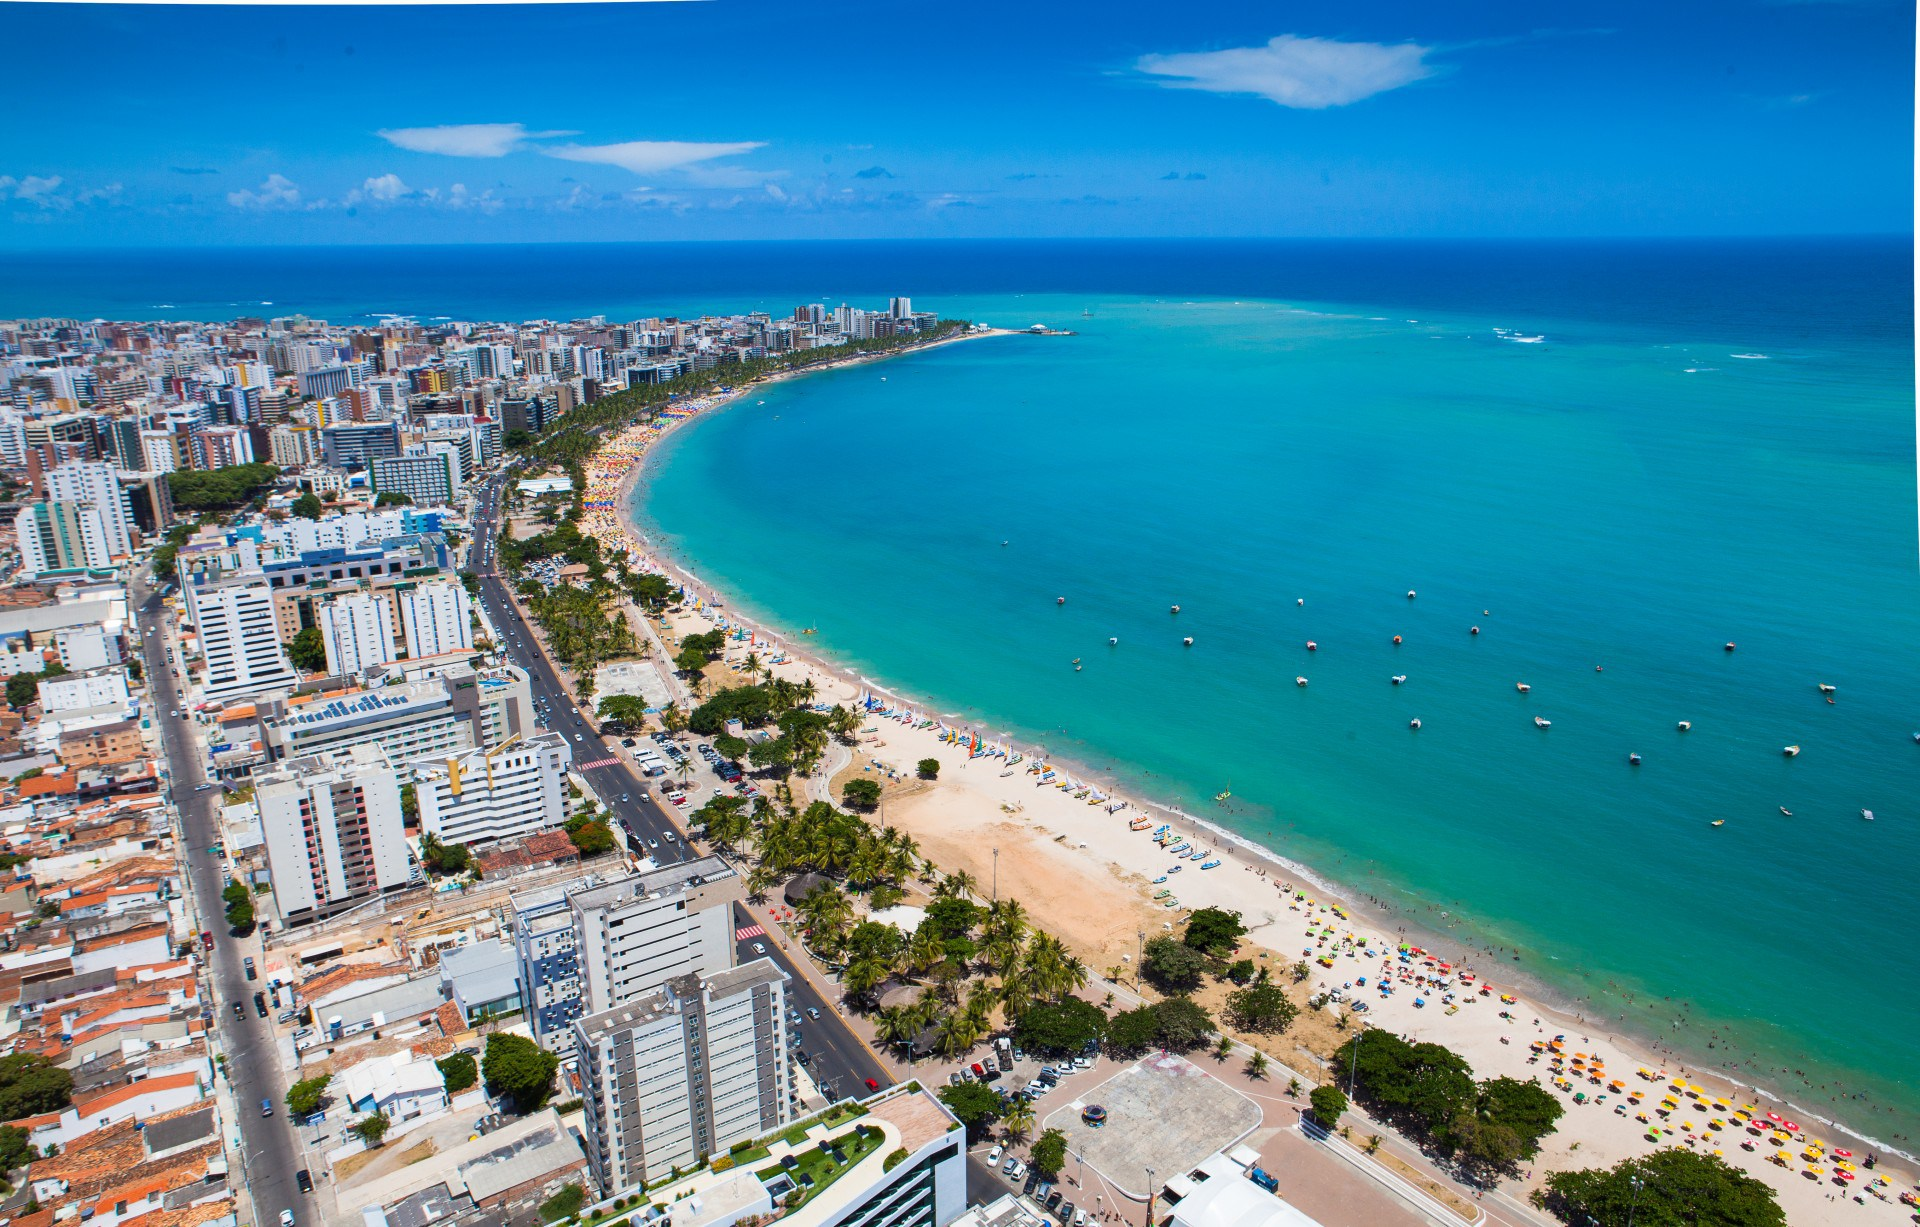
\includegraphics[width=\textwidth]{maceio.jpg}
	\caption{Paraíso das águas.}
\end{figure}

\lipsum[3-5]

\section{Conclusão}
\lipsum[1]

\bibliographystyle{plain}
\begin{thebibliography}{1}
\bibitem{Flusser}
J.~Flusser and T.~Suk.
\newblock Pattern recognition by affine moment invariants.
\newblock {\em Pattern Recognition}, 26:167--174, 1993.

\bibitem{Hu}
M.~K. Hu.
\newblock Visual pattern recognition by moment invariants.
\newblock {\em IRE Transactions on Information Theory}, IT-8:179--187, 1962.
\end{thebibliography}

\end{multicols}
\end{document}